\documentclass[crop,tikz]{standalone}
\tikzstyle{bag} = [align=center]
\usetikzlibrary{positioning}
\usetikzlibrary{arrows.meta}

\begin{document}
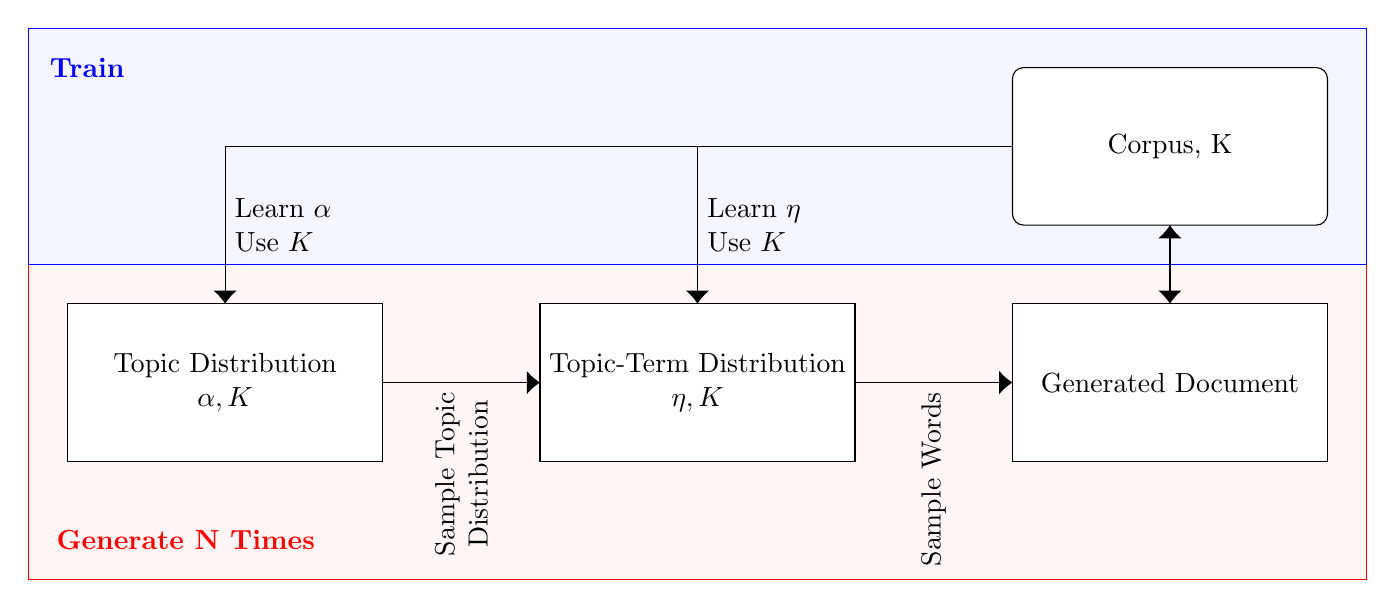
\begin{tikzpicture}[grow=right]
    \draw[red, fill=red!4] (-0.5, -3.5) rectangle (16.5, 0.5);
    \draw[blue, fill=blue!4] (-0.5, 0.5) rectangle (16.5, 3.5);

    \node[align=left, red] at (1.5, -3) {\textbf{Generate N Times}};
    \node[align=left, blue] at (.25, 3) {\textbf{Train}};

    \draw[fill=white] (0, -2) rectangle (4,0) node[bag, pos=.5] {Topic Distribution\\$\alpha, K$};
    \draw[fill=white] (6, -2) rectangle (10,0) node[bag, pos=.5] {Topic-Term Distribution\\$\eta, K$};
    \draw[fill=white] (12, -2) rectangle (16,0) node[bag, pos=.5] {Generated Document};
    \draw[rounded corners, fill=white] (12, 1) rectangle (16,3) node[bag, pos=.5] {Corpus, K};

    \draw[-{Latex[width=3mm]}] (4, -1) -- (6, -1) node[pos=.5, above, rotate=90, anchor=east, bag] {Sample Topic\\Distribution};
    \draw[-{Latex[width=3mm]}] (10, -1) -- (12, -1)  node[pos=.5, above, rotate=90, anchor=east] {Sample Words};

    \draw[-{Latex[width=3mm]}] (12, 2) -- (8, 2) -- (8, 0) node[pos=.5, right, align=left] {Learn $\eta$ \\ Use $K$};
    \draw[-{Latex[width=3mm]}] (12, 2) -- (2, 2) -- (2, 0) node[pos=.5, right, align=left] {Learn $\alpha$ \\ Use $K$};
    \draw[{Latex[width=3mm]}-{Latex[width=3mm]}] (14, 0) -- (14, 1);
\end{tikzpicture}
\end{document}